\section{Highest Locker Priority}
In this section, I will explain about Highest Locker Priority protocol.

\subsection{Definition}

Highest Locker Priority (HLP) is the improvement of the previous protocol to allow the highest priority task $\tau_{i}$ that doesn't use resource $R_{k}$ to interrupt the lower priority task $\tau_{j}$ that use the resource, $R_{k}$ by limiting the raised priority of the task $\tau_{j}$. So, 
 
\begin{equation}
   \citeequation{p_{j}(R_{k})=\underset{h}{\mathrm{max}} \{P_{h}| \tau_{h} \text{   uses } R_{k}\}}{b5}\label{eq1}
\end{equation}

where the priority of task, $\tau_{j}$ that are currently accessing the resource, $R_{k}$ is increased to the maximum only among the tasks that want to access the resource. This dynamic priority then set back to its nominal value $P_{j}$ when the task leaves its critical section. The maximum raised priority of a task $\tau_{j}$ is called priority ceiling $ C(R_{k}) $ and computed off-line.  The maximum priority $ C(R_{k}) $ of the tasks sharing $ R_{k} $ is the computed online such

\begin{equation}
\citeequation{C(R_{k})\stackrel{def}{=}\underset{h}{\mathrm{max}} \{P_{h}| \tau_{h}\text{  uses }  R_{k}\}}{b5}\label{eq2}
\end{equation}

Since the priority of lower priority task $\tau_{j}$ is raised as soon as the task entering $ R_{k} $, this protocol also known as Immediate Priority Ceiling. This protocol can be visualized as in  ``Fig. \ref{fig:Example_of_schedule_under_HLP}'' where task $ \tau_{1} $ have the highest priority and task $ \tau_{3} $ is the first task arrived.

\begin{figure}[ht]
    \centering
    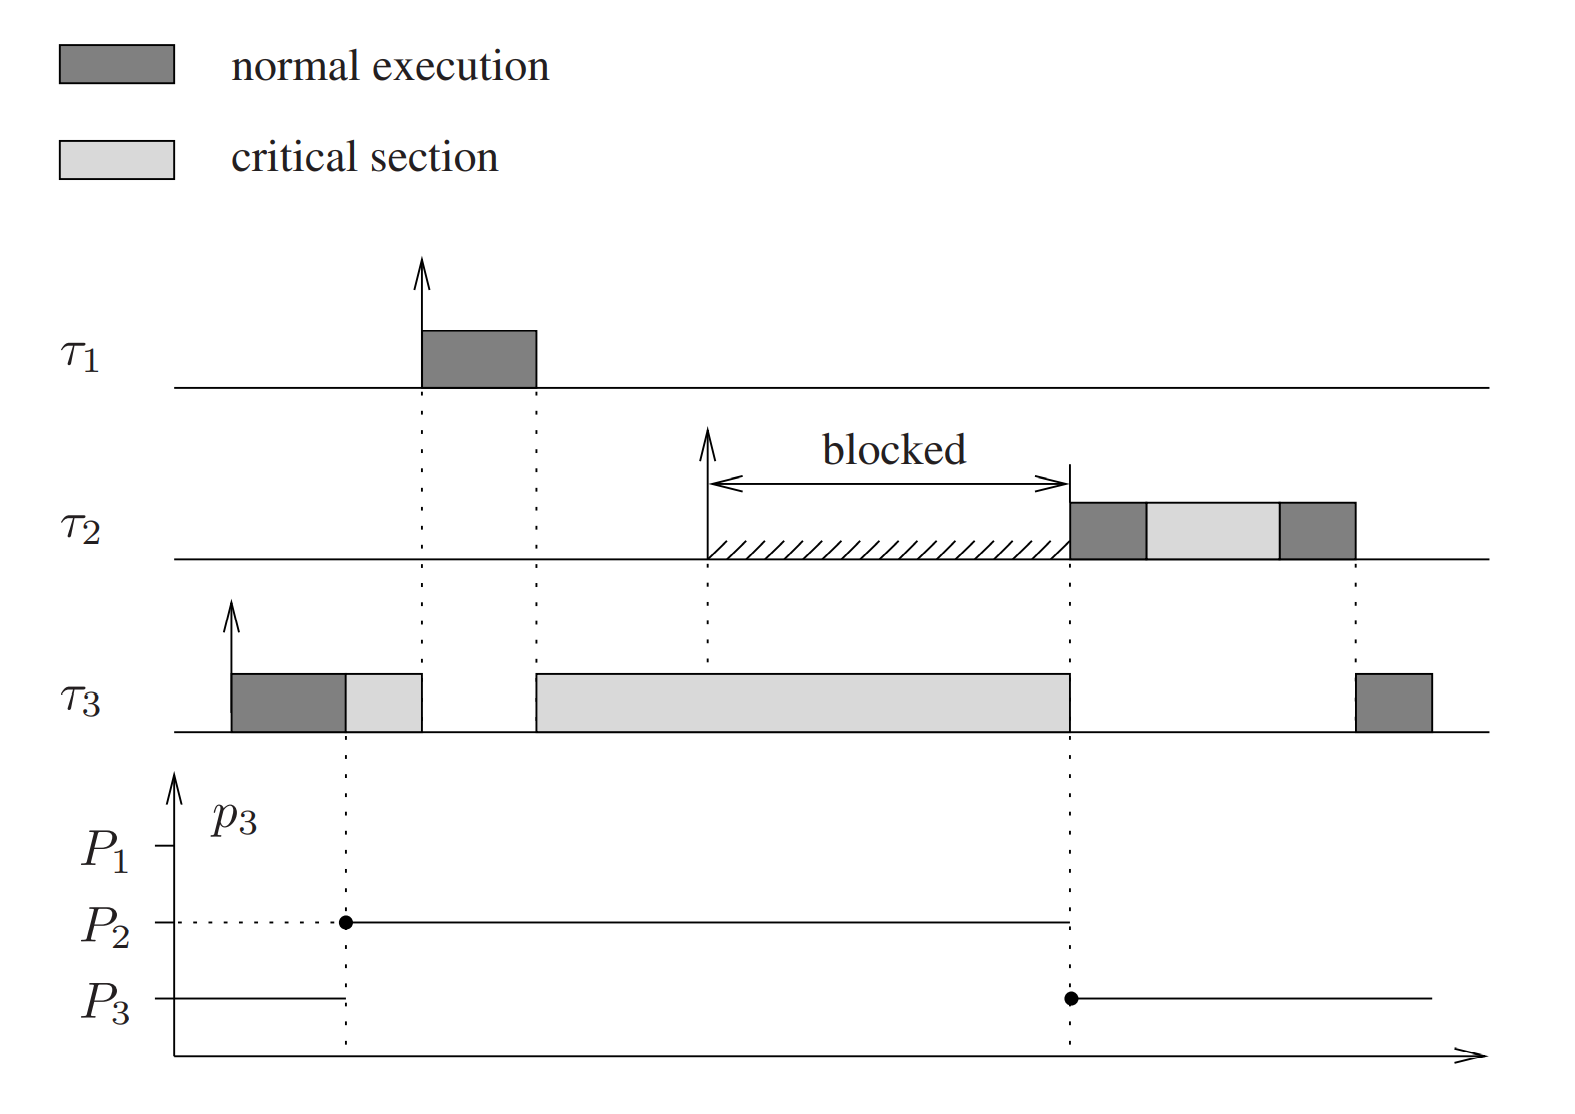
\includegraphics[width=0.5\textwidth]{Example_of_schedule_under_HLP}
    \caption{ Example of schedule under HLP, where $ p3 $ is raised at the level $ C(R) = P_{2} $ as soon as $ \tau_{3} $ starts using resource R \cite{b5}}
    \label{fig:Example_of_schedule_under_HLP}
\end{figure}

 
\subsection{Blocking Time Computation}

The total of critical section of lower priority task $\tau_{j}$ blocking a higher priority task $\tau_{i}$ is reduced by adding a new parameter as shown below. Means that the highest priority task that did not want to use the resource could not be blocked by the lower priority task that are currently using the resource.

\begin{equation}
\citeequation{\gamma_{i}=\{Z_{j,k} | P_{j}<P_{i} \text{   and } C(R_{k})\geq P_{i} \}}{b5}\label{eq3}
\end{equation}

According to \cite{b5}---``Under HLP, a task $ \tau_{i} $ can be blocked, at most, for the duration of a single critical section belonging to the set $ \gamma_{i} $".  

As shown in ``Fig. \ref{fig:Example_of_schedule_under_HLP}'', $ \tau_{i} $ can be blocked at maximum once, means that

\begin{equation}
\citeequation{B_{i}(R_{k})=\underset{j,k}{\mathrm{max}} \{ \delta_{j,k}-1 | Z_{j,k} \in \gamma_{i}\}}{b5}\label{eq4}  
\end{equation}

We need to minus one unit of time because the lower priority task $ \tau_{j} $ needs to access $ R_{k} $ at least one unit of time earlier than $ \tau_{i} $ to block it.

\subsection{Implementation Strategies} 

According to \cite{b6}---``Fewer RTOSs support the Highest Locker Pattern more than the basic Priority Inheritance Pattern. The implementation of this pattern  is fairly straightforward, with the addition of priority ceiling attributes in the Shared Resource. When the mutex is locked, it must notify the Scheduler to elevate the priority of the locking task to that resource's priority ceiling."

\subsection{Sample Model} 

In this section, I will explain the sample model of HLP that I made. Our aim now is to solve the problem in ``Fig. \ref{fig:sample_model_problem_npp}'' by applying HLP. As the result, the dynamic priority of task that currently accessing the resource, $ R_{d}$, which is the display is risen to the highest only among the tasks that want to access the resource, $ R_{d}$. This solution is illustrated in ``Fig. \ref{fig:sample_model_with_hlp}''. So, the task $ \tau_{t}$ can be preempted by the highest priority task, the alarm task, $\tau_{a}$ even though the task is currently accessing the resource $ R_{d}$.


\begin{figure}[ht]
    \centering
    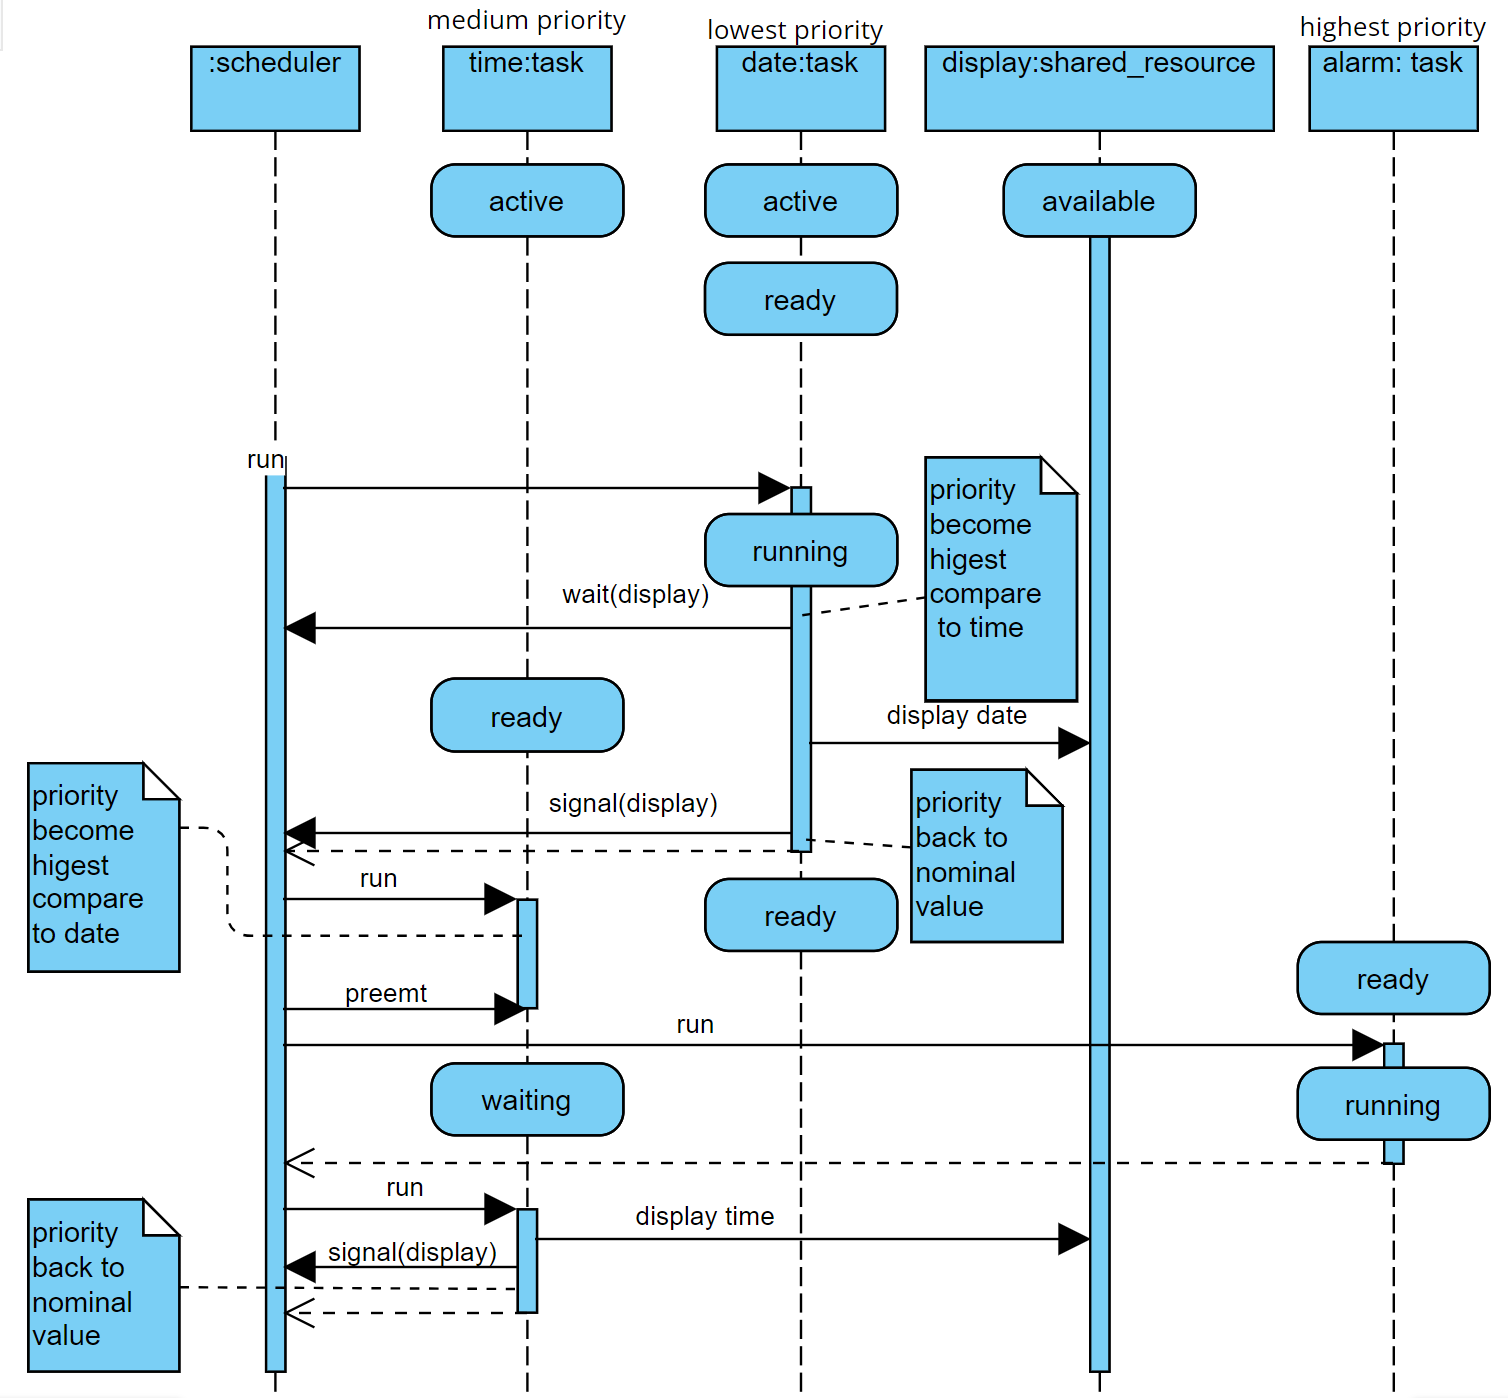
\includegraphics[width=0.5\textwidth]{sample_model_with_hlp}
    \caption{Sample model with HLP}
    \label{fig:sample_model_with_hlp}
\end{figure}


\subsection{Problem Arise}

As claimed by \cite{b5}---``despite the fact that this algorithm improves the previous algorithm, it still could produce some unnecessary blocking. This algorithm block a task at the time it attempts, before it actually require a resource \cite{b5}. If a critical section is contained only in one branch of a conditional statement, then the task could be unnecessarily blocked, since during execution it could take the branch without the resource."
 










